\mbox{$\displaystyle $\,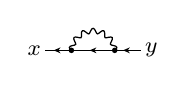
\begin{tikzpicture}[x=0.550cm, y=0.550cm, line width=0.450pt, baseline={([yshift=-0.6ex]0,0)}]
  \draw (0.500,0.000) -- (-0.500,0.000);
  \fill (-0.079,0.000) -- (0.079,-0.068) -- (0.028,0.000) -- (0.079,0.068) -- cycle;
  \draw plot[smooth, tension=0.7] coordinates {(-0.500,0.000) (-0.537,0.035) (-0.548,0.069) (-0.524,0.095) (-0.476,0.110) (-0.427,0.121) (-0.401,0.138) (-0.405,0.168) (-0.427,0.213) (-0.445,0.260) (-0.441,0.296) (-0.407,0.308) (-0.357,0.301) (-0.308,0.290) (-0.278,0.293) (-0.268,0.322) (-0.269,0.372) (-0.265,0.423) (-0.245,0.453) (-0.209,0.450) (-0.167,0.422) (-0.128,0.390) (-0.099,0.380) (-0.078,0.402) (-0.057,0.447) (-0.031,0.491) (0.000,0.509) (0.031,0.491) (0.057,0.447) (0.078,0.402) (0.099,0.380) (0.128,0.390) (0.167,0.422) (0.209,0.450) (0.245,0.453) (0.265,0.423) (0.269,0.372) (0.268,0.322) (0.278,0.293) (0.308,0.290) (0.357,0.301) (0.407,0.308) (0.441,0.296) (0.445,0.260) (0.427,0.213) (0.405,0.168) (0.401,0.138) (0.427,0.121) (0.476,0.110) (0.524,0.095) (0.548,0.069) (0.537,0.035) (0.500,0.000)};
  \draw (-0.500,0.000) -- (-1.100,0.000);
  \fill (-0.909,0.000) -- (-0.751,-0.068) -- (-0.802,0.000) -- (-0.751,0.068) -- cycle;
  \draw (0.500,0.000) -- (1.100,0.000);
  \fill (0.691,0.000) -- (0.849,-0.068) -- (0.798,0.000) -- (0.849,0.068) -- cycle;
  \fill (-0.500,0.000) circle (0.064);
  \fill (0.500,0.000) circle (0.064);
  \node[font=\footnotesize, inner sep=0pt, anchor=0] at (-1.190,0.000) {$x$};
  \node[font=\footnotesize, inner sep=0pt, anchor=180] at (1.190,0.000) {$y$};
\end{tikzpicture}}
\diagramgap
\mbox{$\displaystyle -\,$\,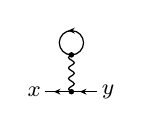
\begin{tikzpicture}[x=0.550cm, y=0.550cm, line width=0.450pt, baseline={([yshift=-0.6ex]0,0)}]
  \draw plot[smooth, tension=0.7] coordinates {(0.000,0.000) (-0.046,0.030) (-0.066,0.061) (-0.046,0.091) (0.000,0.121) (0.046,0.152) (0.066,0.182) (0.046,0.212) (0.000,0.243) (-0.046,0.273) (-0.066,0.304) (-0.046,0.334) (0.000,0.364) (0.046,0.395) (0.066,0.425) (0.046,0.455) (0.000,0.486) (-0.046,0.516) (-0.066,0.546) (-0.046,0.577) (0.000,0.607) (0.046,0.638) (0.066,0.668) (0.046,0.698) (0.000,0.729) (-0.046,0.759) (-0.066,0.789) (-0.046,0.820) (0.000,0.850)};
  \draw (0.000,0.850) arc[start angle=270.000, end angle=630.000, radius=0.280];
  \fill (-0.079,1.410) -- (0.079,1.342) -- (0.028,1.410) -- (0.079,1.478) -- cycle;
  \draw (0.000,0.000) -- (-0.600,0.000);
  \fill (-0.409,0.000) -- (-0.251,-0.068) -- (-0.302,0.000) -- (-0.251,0.068) -- cycle;
  \draw (0.000,0.000) -- (0.600,0.000);
  \fill (0.191,0.000) -- (0.349,-0.068) -- (0.298,0.000) -- (0.349,0.068) -- cycle;
  \fill (0.000,0.000) circle (0.064);
  \fill (0.000,0.850) circle (0.064);
  \node[font=\footnotesize, inner sep=0pt, anchor=0] at (-0.690,0.000) {$x$};
  \node[font=\footnotesize, inner sep=0pt, anchor=180] at (0.690,0.000) {$y$};
\end{tikzpicture}}
\diagramgap
\mbox{$\displaystyle +\,$\,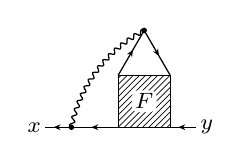
\begin{tikzpicture}[x=0.550cm, y=0.550cm, line width=0.450pt, baseline={([yshift=-0.6ex]0,0)}]
  \draw (-0.600,-0.600) -- (-1.680,-0.600);
  \fill (-1.219,-0.600) -- (-1.061,-0.668) -- (-1.112,-0.600) -- (-1.061,-0.532) -- cycle;
  \draw (0.000,1.635) -- (0.600,0.600);
  \fill (0.340,1.049) -- (0.319,1.220) -- (0.286,1.141) -- (0.202,1.152) -- cycle;
  \draw (-0.600,0.600) -- (0.000,1.635);
  \fill (-0.260,1.186) -- (-0.398,1.083) -- (-0.314,1.094) -- (-0.281,1.015) -- cycle;
  \draw plot[smooth, tension=0.7] coordinates {(-1.680,-0.600) (-1.709,-0.570) (-1.718,-0.544) (-1.699,-0.524) (-1.660,-0.509) (-1.621,-0.494) (-1.602,-0.475) (-1.610,-0.449) (-1.638,-0.418) (-1.665,-0.387) (-1.672,-0.360) (-1.652,-0.342) (-1.613,-0.329) (-1.573,-0.316) (-1.553,-0.298) (-1.560,-0.272) (-1.585,-0.240) (-1.610,-0.207) (-1.616,-0.180) (-1.595,-0.162) (-1.555,-0.151) (-1.515,-0.141) (-1.494,-0.124) (-1.499,-0.098) (-1.522,-0.064) (-1.546,-0.030) (-1.550,-0.002) (-1.528,0.014) (-1.487,0.022) (-1.447,0.030) (-1.424,0.046) (-1.428,0.072) (-1.450,0.108) (-1.471,0.143) (-1.474,0.171) (-1.451,0.186) (-1.410,0.192) (-1.369,0.197) (-1.346,0.212) (-1.348,0.239) (-1.367,0.275) (-1.386,0.312) (-1.388,0.339) (-1.364,0.353) (-1.322,0.357) (-1.281,0.360) (-1.257,0.373) (-1.258,0.400) (-1.275,0.437) (-1.292,0.475) (-1.292,0.503) (-1.267,0.515) (-1.226,0.516) (-1.185,0.517) (-1.160,0.528) (-1.159,0.555) (-1.174,0.594) (-1.189,0.633) (-1.187,0.660) (-1.162,0.671) (-1.120,0.670) (-1.079,0.668) (-1.054,0.678) (-1.051,0.705) (-1.064,0.745) (-1.077,0.784) (-1.074,0.811) (-1.048,0.821) (-1.006,0.817) (-0.965,0.813) (-0.939,0.822) (-0.935,0.849) (-0.946,0.889) (-0.956,0.929) (-0.951,0.956) (-0.925,0.964) (-0.884,0.958) (-0.843,0.952) (-0.817,0.959) (-0.811,0.985) (-0.820,1.026) (-0.828,1.066) (-0.821,1.093) (-0.794,1.100) (-0.754,1.091) (-0.713,1.083) (-0.687,1.088) (-0.679,1.114) (-0.686,1.155) (-0.691,1.196) (-0.683,1.223) (-0.656,1.228) (-0.616,1.217) (-0.576,1.206) (-0.549,1.210) (-0.541,1.236) (-0.544,1.277) (-0.548,1.318) (-0.538,1.344) (-0.511,1.347) (-0.471,1.335) (-0.432,1.321) (-0.405,1.324) (-0.395,1.349) (-0.396,1.390) (-0.397,1.432) (-0.386,1.457) (-0.359,1.459) (-0.320,1.444) (-0.282,1.428) (-0.255,1.429) (-0.243,1.454) (-0.242,1.495) (-0.241,1.536) (-0.228,1.561) (-0.200,1.561) (-0.163,1.544) (-0.125,1.526) (-0.098,1.526) (-0.085,1.549) (-0.082,1.591) (-0.078,1.632) (-0.064,1.656) (-0.037,1.654) (0.000,1.635)};
  \draw (0.000,0.000) -- (-0.600,0.600);
  \draw (0.000,0.000) -- (-0.600,-0.600);
  \draw (0.000,0.000) -- (0.600,-0.600);
  \draw (0.000,0.000) -- (0.600,0.600);
  \draw (-1.680,-0.600) -- (-2.280,-0.600);
  \fill (-2.089,-0.600) -- (-1.931,-0.668) -- (-1.982,-0.600) -- (-1.931,-0.532) -- cycle;
  \draw (0.600,-0.600) -- (1.200,-0.600);
  \fill (0.791,-0.600) -- (0.949,-0.668) -- (0.898,-0.600) -- (0.949,-0.532) -- cycle;
  \fill[white] (-0.600,-0.600) rectangle (0.600,0.600);
  \draw[line width=0.248pt] (-0.600,0.531) -- (-0.531,0.600) (-0.600,0.390) -- (-0.390,0.600) (-0.600,0.249) -- (-0.249,0.600) (-0.600,0.107) -- (-0.107,0.600) (-0.600,-0.034) -- (0.034,0.600) (-0.600,-0.176) -- (0.176,0.600) (-0.600,-0.317) -- (0.317,0.600) (-0.600,-0.459) -- (0.459,0.600) (-0.600,-0.600) -- (0.600,0.600) (-0.459,-0.600) -- (0.600,0.459) (-0.317,-0.600) -- (0.600,0.317) (-0.176,-0.600) -- (0.600,0.176) (-0.034,-0.600) -- (0.600,0.034) (0.107,-0.600) -- (0.600,-0.107) (0.249,-0.600) -- (0.600,-0.249) (0.390,-0.600) -- (0.600,-0.390) (0.531,-0.600) -- (0.600,-0.531);
  \begin{scope}
  \clip (-0.600,-0.600) rectangle (0.600,0.600);
  \node[font=\footnotesize, inner sep=1.2pt, fill=white, rounded corners=2pt] at (0.000,0.000) {$F$};
  \end{scope}
  \draw (-0.600,-0.600) rectangle (0.600,0.600);
  \fill (-1.680,-0.600) circle (0.064);
  \fill (0.000,1.635) circle (0.064);
  \node[font=\footnotesize, inner sep=0pt, anchor=0] at (-2.370,-0.600) {$x$};
  \node[font=\footnotesize, inner sep=0pt, anchor=180] at (1.290,-0.600) {$y$};
\end{tikzpicture}}
